%
% File acl2014.tex
%
% Contact: koller@ling.uni-potsdam.de, yusuke@nii.ac.jp
%%
%% Based on the style files for ACL-2013, which were, in turn,
%% Based on the style files for ACL-2012, which were, in turn,
%% based on the style files for ACL-2011, which were, in turn, 
%% based on the style files for ACL-2010, which were, in turn, 
%% based on the style files for ACL-IJCNLP-2009, which were, in turn,
%% based on the style files for EACL-2009 and IJCNLP-2008...
%% Based on the style files for EACL 2006 by 
%%e.agirre@ehu.es or Sergi.Balari@uab.es
%% and that of ACL 08 by Joakim Nivre and Noah Smith

\documentclass[11pt]{article}
\usepackage{acl2014}
\usepackage{times}
\usepackage{url}
\usepackage{latexsym}
\usepackage{amsmath}
\usepackage{xspace}

\usepackage[usenames,dvipsnames,svgnames,table]{xcolor}
\usepackage{soul}

\usepackage{algorithm}
\usepackage[noend]{algpseudocode}
\usepackage{graphicx}
\usepackage{caption}
\usepackage{subcaption}

\usepackage{tikz-dependency}

\usepackage[usenames,dvipsnames,svgnames,table]{xcolor}  % allows better color names
\usepackage{todonotes}   % insert [disable] to disable all notes
% Note that these macros accept optional arguments such as 
% [size=\small,bordercolor=red].
\newcommand{\Note}[4][]{\todo[author=#2,color=#3,fancyline,#1]{#4}}
\newcommand{\noteJH}[2][]{\Note[#1]{JH}{blue!40}{#2}}
\newcommand{\noteJE}[2][]{\Note[#1]{JE}{green!40}{#2}}   
\newcommand{\notewho}[3][]{\Note[#1]{#2}{orange!40}{#3}}  % extra arg with miscellaneous author
\newcommand{\NoteJH}[2][]{\noteJH[inline,#1]{#2}}
\newcommand{\NoteJE}[2][]{\noteJE[inline,#1]{#2}}
\newcommand{\Notewho}[3][]{\notewho[inline,#1]{#2}{#3}}  % extra arg with miscellaneous author

% \newcommand{\root}{\texttt{\$}}

\title{Deriving Multi-Headed Projective Dependency Parses \\ from Link Grammar Parses}
% Oriented link grammar: Creating a multi-headed dependency corpus.

% \author{Juneki Hong and Jason Eisner\\
%   Department of Computer Science \\
%   Johns Hopkins University \\
%   Baltimore, MD 21218, USA \\ 
%   {\tt \{juneki,jason\}@cs.jhu.edu} \\
% }

\date{}

\begin{document}
\maketitle

\begin{abstract}
Under multi-headed dependency grammar, a parse is a DAG rather than a tree.  Such formalisms can be more syntactically and semantically expressive.  However, 
it is hard to train, test, or improve multi-headed parsers because few multi-headed corpora exist, particularly for the projective case.
% OLD
% investigate the benefit of such parsers or to work on making them faster or more accurate.  
To help fill this gap, we observe that link grammar already produces {\em undirected} projective graphs.  
% OLD
% ... produces parses that are similar to multi-headed projective dependency parses, except that the links are undirected. 
We use Integer Linear Programming to assign consistent directions to the labeled links in a corpus of 70,000 \noteJE{fill in the number} parses produced by the Link Grammar Parser, which has broad-coverage hand-written grammars of English as well as Russian and other languages.  We find that such directions can indeed be consistently assigned in a way that yields valid multi-headed dependency parses. The resulting parses in English appear reasonably linguistically plausible, although they are not in general consistent with CoNLL-style parses of the same sentences; we discuss the differences.  
\end{abstract}

\section{Multi-Headed Dependency Parsing}

Dependency parsing maps a sentence to a directed graph whose vertices are the words $1, 2, \ldots, n$ of the sentence along with a distinguished ``root'' vertex 0.  A labeled directed edge $u \stackrel{L}{\rightarrow} v$ or $v \stackrel{L}{\leftarrow} u$ indicates that the ``child'' $v$ is some kind of argument or modifier of its ``parent'' $u$.  The edge label $L$ indicates the specific syntactic or semantic relationship between the two words.  

In the special case $u=0$, the edge designates $v$ as playing some special top-level role in the sentence, e.g., as the main verb.  We disallow $v=0$.

As recently discussed by \newcite{gomezrodriguez-nivre-2013}, one might impose various requirements on the parse graph:
\begin{itemize}
\item {\sc Single-Head}: each word has at most one parent
\item {\sc Acyclic}: there are no directed cycles
\item {\sc Connected}: each pair of words has a undirected path between them
\item {\sc Reachable}: each word can be reached from 0 by a directed path
\item {\sc Planar}: edges may not ``cross'' \\ (if there are edges between $u,v$ and between $i,j$, where $u < i < v$, then $u \leq j \leq v$)
\end{itemize}
It is common to impose all of these requirements at once, leading to a {\em projective dependency parser} that produces projective trees rooted at 0.\footnote{{\sc Projective} basically means {\sc Planar} + {\sc Reachable}.}  However, parsing algorithms can be devised that relax any or all of the requirements \cite{gomezrodriguez-nivre-2013}.  

In this paper, we are interested in relaxing the {\sc Single-Head} requirement while preserving all the others.  This means that the parse can have more than $n$ edges, allowing it to express more relationships between words.  In English, for example, here are some constructions that seem to call for a multi-headed analysis.  
\begin{description}
\item[control] In {\em ``Jill likes to skip,''} the word {\em Jill} is the subject of two verbs.  In {\em ``Jill persuaded Jack to skip,''} {\em Jack} is the object of one verb and the subject of another.  Without recognizing this, our parser would miss the syntactic invariants that {\em skip} always has a subject and {\em persuaded} always has an object.  It would also be unable to exploit the selectional preferences of both verbs to help disambiguate the parse.  This is why we prefer to make the parser aware of multi-headedness, rather than using a single-headed parser and then extracting the additional semantic roles from its output.
\item[relativization] In {\em ``The boy that Jill skipped with fell down,''} the word {\em boy} is the object of {\em with} as well as the subject of {\em fell}.  Without recognizing this, we would miss the syntactic invariant that {\em with} always has an object.  
\item[conjunction] In {\em ``Jack and Jill went up the hill,''} {\em Jack} and {\em Jill} serve as the two arguments to {\em and}, but they are also semantically subjects of {\em went}.  Without recognizing this, we would have no (local) reason for expecting the arguments of {\em and} to be nouns.
\end{description}

In linguistics, it is common to analyze some of these structures using trees with ``empty categories.''  The subject of {\em skip} is taken to be a silent morpheme {\em PRO}:
{\em ``Jill$_i$ likes PRO$_i$ to skip.''}  However, this is no longer a tree if one considers the implicit undirected edge between {\em Jill} and {\em PRO} (denoted by their shared index $i$).  Our simpler representation contracts this coreference edge, eliminating {\em PRO} and creating a {\em Jill} $\leftarrow$ {\em skip} link.  

\section{Link Grammars}

A few past NLP papers have explored multi-headed dependency parsing \cite{buchkromann-2006,mcdonald-pereira-2006,sagae-tsujii-2008,gomezrodriguez-nivre-2013}.  Unfortunately, there seem to be no annotated corpora in this form other than the Danish Dependency Treebank \cite{kromann-2003}; researchers have sometimes converted corpora from other formats such as HPSG.  

All of these options result in non-projective parses, so the parsers must use non-projective or pseudo-projective algorithms.

It seems at first that no one has worked out annotation conventions for {\em projective} multi-headed dependency parsing.  However, this is not quite true.  Link Grammar \cite{SleatorTemperly91} is a grammar-based formalism for projective dependency parsing with {\em undirected} links.  It produces undirected connected planar graphs.  The annotation conventions are implicit in the detailed Link Grammar lexicon,%
\footnote{\url{http://www.abisource.com/projects/link-grammar/dict/introduction.html}.  The 122 link types in the English lexicon are documented at \url{http://www.abisource.com/projects/link-grammar/dict/summarize-links.html}.} 
which specifies for every word a constraint on the {\em sequence} of labeled leftward and rightward edges attached to it.  As remarked by \newcite{eisner-2000-iwptbook}, this is analogous to dependency grammar's use of head automata to constrain a word's sequence of left and right children.  For example, in {\em ``The boy that Jill skipped with fell down,''} the word {\em with} uses a lexical entry that requires it to link to a governing verb to the left, an extracted object farther to the left, and nothing to the right.

Given a link grammar parse, it would be straightforward to convert it to an acyclic dependency parse by orienting all edges rightward.  However, the result may violate the {\sc Reachability} constraint.  Instead we could orient all edges by depth-first search from the root node, which yields a DAG satisfying all our constraints.  However, this might result in inconsistent annotation conventions, with some \texttt{S} links pointing from subject to verb and others from verb to subject.  

We supposed that the link grammar lexicon designers actually had a consistent direction in mind for each edge type.  We would expect verbs to point to their subject arguments in dependency grammar, and so we surmise that all \texttt{S} links are intended to point leftward (from verb to subject: {\em ``Jack $\stackrel{\texttt{S}}{\leftarrow}$ is falling''}).  The link grammar designers take care to use a distinct \texttt{SI} label in cases of subject-verb inversion, and we surmise that \texttt{SI} links are intended to point rightward (again from verb to subject: {\em ``Jack $\stackrel{\texttt{SI}}{\rightarrow}$ is falling''}).

Our goal in this paper is to recover these implicit directions by global optimization.  We seek a fixed mapping from labels to directions such that we can interpret link grammar parses as directed dependency parses that satisfy all of our constraints.

Our first thought was to seek a direction mapping such that no parsed word sequence allowed by the link grammar lexicon could possibly violate our constraints after directions were imposed.  This is a well-defined constraint programming problem.  For example, to prevent cyclicity, we would require (roughly speaking) that no word type could follow a sequence of directed rightward links through other word types and then a leftward link back to itself.  

However, working directly with the link grammar lexicon format is somewhat tricky.  We also feared that there would not be a perfect solution---for example, because of errors in the lexicon, or linguistically unnatural word sequences not anticipated by the grammar designers.  In this case it would not be clear how to relax our constraints.

Thus, we chose to use a sample of {\em actual} sentences parsed by the link grammar, and to seek a direction mapping so that {\em these} parses would not violate our constraints after directions were imposed.  If no such mapping exists, then we are willing to orient a few edge tokens in the wrong direction to ensure that the parses are still well-formed---but we minimize the number of such violations.  In this way, the empirical distribution of sentences guides our assignment of directions.  The resulting directed corpus can be used for research on multi-headed dependency parsing.

% Link grammars are a grammatical system equivalent to context-free grammars that assign linking requirements to every given word. A link parser then tries to satisfy all of these requirements for every word of a sentence while still maintaining planarity. The resulting links describe the relationships between constituents in a parse. 

% The link grammar is based on a set of handwritten dictionaries. Instead of going through these dictionaries, we learned the grammar using an ILP. This approach also potentially allows us to analyze link grammar dictionaries other than English. \todo{explore other link grammar dictionaries} 

% \NoteJE{what statistics does it use?  what languages are available}

% Link parsing in contrast produces a multiheaded planar graph with undirected edges, where every edge has a label describing the relationship between two constituents in a parse. In this paper we explore whether these relationships include dependencies, and whether the multiheadedness of the link grammar offers additional dependency relationships not found in other corpora.

%about 20\% 

% Dependency parsing is the task of mapping a sentence to a projective (not always projective?) directed acyclic tree. Link parsing in contrast produces a multiheaded planar graph with undirected edges, where every edge has a label describing the relationship between two constituents in a parse. In this paper we explore whether these relationships include dependencies. To determine the directional dependencies within the link edge labels we will use integer linear programming, encoding the problem in the Zimpl little language \cite{Koch2004}. It turns out that the link parses roughly only match half of the conll dependency corpus. However this is because \todo{}. 

\section{Integer Linear Programming}
We formulate an ILP to find the minimal set of link type to directionality assignments that would directionalize all the links in a set of link grammar parses, while still mandating that all of the resulting dependency parses would be connected DAGs, and with all the nodes reachable from the root. 

For every encountered label we generate two boolean label/direction variables (e.g. label/left, label/right). Setting one of these variables to \textsc{true} allows the label type to only go in the specified direction, while setting both would allow the label to go in either way.
The objective is to minimize the number of label/direction variables set to \textsc{true}, while still satisfying acyclicity and reachability constraints. The encoding was written in the Zimpl little language \cite{Koch2004} and solved using the SCIP Optimization Suite\cite{achterberg2009scip}.

\todo{cite model minimization papers}

\begin{figure*}
  \small
  \begin{align*}
    \text{Sets:}&&\\
    &\textsc{link}_{i,j,\textsc{label},\textsc{sentence}} \in \textsc{links} &\\
    &\textsc{label} \in \textsc{labels}&\\ 
    &\textsc{dir} = \{\textsc{left}, \textsc{right}\} &\\
    \text{Params:}&&\\
    &\textsc{m}_\textsc{length} = \max (\forall{\textsc{link}_{i,j,\textsc{sentence}}} \max(i,j)) &\\
    %&\textsc{count}_{\textsc{label}, \textsc{dir}} = \sum_{\textsc{link}_{\textsc{label},\textsc{dir}}}1 &\\
    &\textsc{cost}_{\textsc{label}} = \frac{100}{ \sum_{\textsc{link}_{\textsc{label},\textsc{dir}}}1 } &\\
    \text{Variables:}&&\\
    &\textsc{slack}_{\textsc{link}} \geq 0 &\\ 
    &\textsc{depth}_{i,\textsc{sentence}} \geq 0 &\\
    &\textsc{allowed}_{\textsc{label},\textsc{dir}} = \{0,1\}&\\
    &\textsc{arc}_{\textsc{link}} = \{0,1\} &\\
    \text{minimize:}& &\\ 
    &\sum_{\textsc{label}, \textsc{dir}} (\textsc{allowed}_{\textsc{label},\textsc{dir}}) + \textsc{cost}_{\textsc{label}} \cdot \sum_\textsc{link} \textsc{slack}_{\textsc{link}} &\\
    &&\\
    \text{subject to: }& &\\
    &\text{Links go in the allowed directions, except for slack}&\\
    &\forall{\textsc{link}_{i,j,\textsc{label}}}: 1-\textsc{arc}_{\textsc{link}} \leq \textsc{allowed}_{\textsc{label}, \textsc{left}} + \textsc{slack}_{\textsc{link}} &\\
    &\forall{\textsc{link}_{i,j,\textsc{label}}}: \textsc{arc}_{\textsc{link}} \leq \textsc{allowed}_{\textsc{label}, \textsc{right}} + \textsc{slack}_{\textsc{link}} &\\
    &\text{Depth constraints for acyclicity}&\\
    &\forall{\textsc{link}_{i,\textsc{sentence}}}: \textsc{depth}_{\text{root},\textsc{sentence}} \leq \textsc{depth}_{i,\textsc{sentence}} &\\
    &\forall{\textsc{link}_{i,j,\textsc{sentence}}}: \textsc{depth}_{i,\textsc{sentence}} + \textsc{m}_\textsc{length}\cdot\textsc{arc}_{i,j,\textsc{sentence}} \geq \textsc{depth}_{j,\textsc{sentence}} + 1 &\\
    &\forall{\textsc{link}_{i,j,\textsc{sentence}}}: \textsc{depth}_{j,\textsc{sentence}} + \textsc{m}_\textsc{length}\cdot(1-\textsc{arc}_{i,j,\textsc{sentence}}) \geq \textsc{depth}_{i,\textsc{sentence}} + 1 &\\
    &\text{Every token has a parent}&\\
    &\forall{\textsc{link}_{i \neq \textsc{root},\textsc{sentence}}}: \sum_{\textsc{link}_{i,j,\textsc{sentence}}} (1-\textsc{arc}_{i,j,\textsc{sentence}}) + \sum_{\textsc{link}_{j,i,\textsc{sentence}}}(\textsc{arc}_{j,i,\textsc{sentence}}) \geq 1&\\
  \end{align*}
  \caption{\small The ILP formulation.}
\end{figure*}


\subsection{Slack}
We introduced slack such that the link types were allowed to deviate from the majority one percent of the time before the ILP would assign both label/direction variables to \textsc{true}. This allows for flexibility against noise in the link parser's label assignments, balanced with allowing for both directions to be assigned if necessary.


\section{Experiments and Results}
To evaluate ...

We generated link parses using the AbiWord/CMU link grammar parser version 5.0.8 \cite{LINKPARSER-2014}. 

The experiments were conducted on Russian and English sentences.
The Russian sentences were taken from a part of the Russian National Corpus (about 75,000 sentences)\noteJH{cite?}. 
The English sentences were taken from the conll bnews training data (about 60,000 sentences)\noteJH{cite?}. We were able to compare the resulting English link dependency data with the original conll to analyze the differences. 

We publish the final link type to direction assignments so that anyone can easily turn a link parse into a dependency parse.


We report on the convergence of the results of our ILP with increasing data. With increasing trials of sentences, we measure how similar the subsequent directional assignments would be with each other. Taking the largest run as the answer key, we compared how much the smaller runs deviated from it. 
We recorded the precision of whether the assignments in the smaller runs could be found in those of the largest run, and similarly the recall of whether the assignments in the largest run could be found in the smaller runs. 

\subsection{Stability of Results}
\begin{figure}[ht!]
  \small
  \centering
  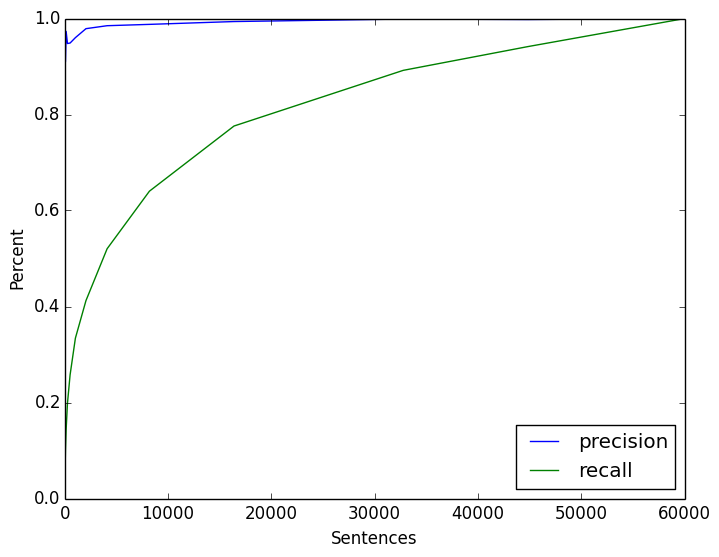
\includegraphics[width=0.9\linewidth, keepaspectratio=true]{figure/precision_recall.png}
  \caption{\small Precision/recall of increasing runs of English and Russian sentences}
\end{figure}


We found that the precision values converged to 100\% while the recall values continued to grow throughout the data. This indicates that the solutions of the previous runs were consistent with the largest run, and as the data increased we would continue to encounter novel link types and incorporate them.


\subsection{Link Corpus Analysis}

\begin{figure*}[ht!]
  \centering
  \begin{subfigure}[b]{0.3233\textwidth}
	\begin{dependency}
		\begin{deptext}
			{\scriptsize PR} \& {\scriptsize VB} \& {\scriptsize RB} \& {\scriptsize VB} \& {\scriptsize .} \\
			it \& did \& n't \& work \& . \\
			- \& v-d \& - \& v \& - \\
		\end{deptext}
		\deproot[edge above, edge style = {blue, dotted}]{2}{\small ROOT}
		\depedge[edge below, edge style = {red, ultra thick}]{1}{2}{Ss}
		\depedge[edge above, edge style = {blue, thick}]{2}{1}{\small SBJ}
		\depedge[edge below, edge style = {red, thick}]{2}{3}{N}
		\depedge[edge above, edge style = {blue, thick}]{2}{3}{\small VMOD}
		\depedge[edge below, edge style = {red, thick}]{2}{4}{I*d}
		\depedge[edge above, edge style = {blue, thick}]{2}{4}{\small VC}
		\depedge[edge above, edge style = {blue, dotted}]{2}{5}{\small P}
		\deproot[edge below, edge style = {red, dotted}]{1}{Wd}
		\deproot[edge below, edge style = {orange, ultra thick}]{4}{WV}
		\deproot[edge below, edge style = {red, dotted}]{5}{Xp}
	\end{dependency}
\end{subfigure}
\begin{subfigure}[b]{0.3233\textwidth}
	\begin{dependency}
		\begin{deptext}
			{\scriptsize DT} \& {\scriptsize NN} \& {\scriptsize VB} \& {\scriptsize JJ} \& {\scriptsize .} \\
			the \& reason \& is \& simple \& . \\
			- \& n \& v \& a \& - \\
		\end{deptext}
		\deproot[edge below, edge style = {red, thick}]{3}{WV}
		\deproot[edge above, edge style = {blue, thick}]{3}{\small ROOT}
		\depedge[edge below, edge style = {red, thick}]{3}{2}{Ss*t}
		\depedge[edge above, edge style = {blue, thick}]{3}{2}{\small SBJ}
		\depedge[edge below, edge style = {red, thick}]{3}{4}{Paf}
		\depedge[edge above, edge style = {blue, thick}]{3}{4}{\small VMOD}
		\depedge[edge above, edge style = {blue, dotted}]{3}{5}{\small P}
		\depedge[edge below, edge style = {red, thick}]{2}{1}{D*u}
		\depedge[edge above, edge style = {blue, thick}]{2}{1}{\small NMOD}
		\deproot[edge below, edge style = {orange, ultra thick}]{2}{Wd}
		\deproot[edge below, edge style = {red, dotted}]{5}{Xp}
	\end{dependency}
\end{subfigure}
\begin{subfigure}[b]{0.3233\textwidth}
	\begin{dependency}
		\begin{deptext}
			{\scriptsize DT} \& {\scriptsize NN} \& {\scriptsize VB} \& {\scriptsize RB} \& {\scriptsize .} \\
			the \& judge \& wrote \& again \& . \\
			- \& n \& v-d \& - \& - \\
		\end{deptext}
		\deproot[edge below, edge style = {red, thick}]{3}{WV}
		\deproot[edge above, edge style = {blue, thick}]{3}{\small ROOT}
		\depedge[edge below, edge style = {red, thick}]{3}{2}{Ss}
		\depedge[edge above, edge style = {blue, thick}]{3}{2}{\small SBJ}
		\depedge[edge below, edge style = {red, thick}]{3}{4}{MVa}
		\depedge[edge above, edge style = {blue, thick}]{3}{4}{\small ADV}
		\depedge[edge above, edge style = {blue, dotted}]{3}{5}{\small P}
		\depedge[edge below, edge style = {red, thick}]{2}{1}{Ds}
		\depedge[edge above, edge style = {blue, thick}]{2}{1}{\small NMOD}
		\deproot[edge below, edge style = {orange, ultra thick}]{2}{Wd}
		\deproot[edge below, edge style = {red, dotted}]{5}{Xp}
	\end{dependency}
\end{subfigure}


  \caption{Example Parses: The top blue arcs represent the conll dependencies, and the bottom red arcs are the directionalized link grammar parses}
  \label{fig:parses}
\end{figure*}





Using the sentences of a dependency corpus as comparison, we find that the link parses do not wholly subsume dependency parses, and that the undirected links match roughly two thirds of the arcs in the conll dependency corpus. \todo{This is because...} 
Of the links that match a corresponding dependency arc we measure whether the direction we chose is the same as the original dependency data. 
Finally, we look to see that given a link label, whether the original conll label can be recovered.


We ran the link parser and our ILP on the english bnews corpus sentences. \footnote{We ignored the link parses that the link parser could not find suitable attachments and returned a disconnected graph. This happened for roughly 19\% of the sentences in the corpus.} 
From this, we generated directionalized multiheaded dependency data to compare with the original conll data.

\begin{figure}[ht!]
  \centering
  \small
  	\begin{tabular}{|l|l|}
		\hline
		Original number of sentences in conll corpus & 4096\\ 
		\hline
		Sentences after discarding disconnected parses & 3303\\ 
		\hline
		Sentences used for experiment and analysis & 2969\\ 
		\hline
	\end{tabular}

  \caption{\small From the original sentences, we discarded disconnected parses for the ILP. From these sentences, we only looked at the complete link parses and discarded sentences with dropped words for our analysis section. About 0.00\% of the non-disconnected sentences contained dropped words.}
\end{figure}

\todo{Fix the caption in the conll analysis sentence chart}

About 78.10\% of the sentences with complete parses had at least one multiheaded word


Compared to the original conll data, the link parses match about half the conll arcs in location and directionality. The mismatches in the other half can be accounted for in the following ways.

\subsection{Blanks}
The link parser will skip and attach no links to words that it failed to recognize from its dictionary. This accounts for about ten percent of the mismatches.

\subsection{Directional Mismatches}
In about 25\% of the cases, the conll arc's corresponding link would be assigned the opposite direction.


\section{Discussion}



\todo{more in the appendix ...}

\NoteJE{We should acknowledge that another option would be to post-process either CoNLL parses or our link parses to automatically add more multi-heading, e.g., to handle control phenomena ("John wants to skip" or "Jane ran for office in order to change the tax laws" should have John/Jane be the subject of two verbs).  However, that requires per-language}

We have a set of 100 parses similar to figure~\ref{fig:parses} in the appendix.



\section{Future Work}

\subsection{Slack Hierarchy}
We would like to introduce slack on the link grammar types such that link types with the same coarse grained label would try and align the same way as the majority in the group, where the preceding capital letters of the link type denote the coarse grained label, while the subscript letters denote further information. This slack would place a prior on rare or never-before seen link types to be assigned in the same way as other similar link types. We think that this will give the ILP better flexibility to handle noise and novel link types while still trying to learn the overall link grammar.





\section{Related Work}



\bibliographystyle{acl2014}
\bibliography{LinksToDAG}





\clearpage
\appendix
\section{English Link Types}

\todo[inline]{A table here that lists each link grammar type together with its
  count, its allowed direction(s), its percentage of majority
  directions by token, and its most common corresponding CoNLL tags
  with percentages.  Readers could cut-and-paste this data to make a 
  cheap post-processor for LG parses.}

\section{Sample English Parses}

\todo[inline]{Show a bunch of English sentences with CoNLL vs.\@ link parses.
  Explain how they were selected and how the results are colorized etc.}

Here we display a set of link parses as further examples


\end{document}
